
\section{Experimentos}
En esta sección, primero realizamos un estudio de ablación sobre las decisiones de diseño de \model y luego adoptamos la mejor configuración para el entrenamiento a gran escala.
\subsection{Ablation Study}
% We explore the \model design space to determine the effectiveness of our model components. We initialize all models based on a strong transformer-based LMM Qwen2-VL-7B \cite{wang2024qwen2}. For all ablation experiments, we use 1M image-caption pairs from PixelProse \cite{singla2024pixels} for pretraining, and employ the LLaVA-Video-178K \cite{zhang2024video} dataset with a total of 1.3M video-instruction pairs for instruction-tuning. Detailed hyperparameter settings can be found in Appendix~\ref{sec:additional_implementation}.
Exploramos el espacio de diseño de \model para determinar la efectividad de los componentes del modelo. Inicializamos todos nuestros modelos a partir de un sólido LMM basado en Transformer preentrenado, Qwen2-VL-7B \cite{wang2024qwen2}. Para todos los experimentos de ablación, seleccionamos aleatoriamente un millón de imágenes de CC12M \cite{changpinyo2021conceptual} y empleamos los captions de PixelProse \cite{singla2024pixels} para el preentrenamiento. Utilizamos el dataset LLaVA-Video-178K \cite{zhang2024video} con un total de 1.3M pares video-instrucción para el instruction-tuning. La configuración detallada de hiperparámetros puede encontrarse en el Apéndice~\ref{sec:additional_implementation}.

\begin{table}[]
\centering
\small
\caption{Resultados del estudio de ablación para las exploraciones del espacio de diseño de \model. ``CA from SA?'' indica si los pesos de cross-attention se inicializan a partir de capas self-attention. ``VidMME'' representa el benchmark Video-MME.}
\setlength\tabcolsep{1.5 pt}
\begin{tabular}{@{}ccccccc@{}}
\toprule
\multirow{4}{*}{\begin{tabular}[c]{@{}c@{}}Model\\ ID\end{tabular}} & \multirow{4}{*}{\begin{tabular}[c]{@{}c@{}}CA\\ from\\ SA?\end{tabular}} & \multirow{4}{*}{\begin{tabular}[c]{@{}c@{}}Mamba\\ Block\\ Type\end{tabular}} & Stage 1 & \multicolumn{3}{c}{Stage 2}                                     \\ \cmidrule(l){4-7} 
                                                                    &                                                                          &                                                                               & G-VEval     & \multicolumn{1}{c}{LVBench} & \multicolumn{1}{c}{VidMME}    & MVBench \\ \cmidrule(l){4-7} 
                                                                    &                                                                          &                                                                               & ref. free   & \multicolumn{1}{c}{test}    & \multicolumn{1}{c}{w/o sub.} & test    \\ \midrule
A                                                                   & \xmark                                                                        & N/A                                                                           & 75.7        & \multicolumn{1}{c}{23.7}    & \multicolumn{1}{c}{47.6}         & 40.9    \\
B                                                                   & \cmark                                                                        & N/A                                                                           & 81.0        & \multicolumn{1}{c}{34.2}    & \multicolumn{1}{c}{51.7}         & 51.8    \\
C                                                                   & \cmark                                                                        & Mamba                                                                         & 81.8        & \multicolumn{1}{c}{34.2}        & \multicolumn{1}{c}{53.4}             & 53.5        \\
D                                                                   & \cmark                                                                        & Mamba-2                                                                       & 82.2        & \multicolumn{1}{c}{35.3}    & \multicolumn{1}{c}{54.1}         & 53.5    \\ \bottomrule
\end{tabular}
\label{tab:ablation_main}
\end{table}

\begin{table}[]
\centering
\small
\caption{Resultados del estudio de ablación del pretraining de modelos \model con un teacher LMM basado en Transformer y una distillation loss.}
\setlength\tabcolsep{6.5 pt}
\begin{tabular}{@{}lclcccc@{}}
\toprule
\multirow{2}{*}{\begin{tabular}[c]{@{}l@{}}Model D\\ + Distill\end{tabular}} & \multicolumn{6}{c}{$\lambda$ value in Stage 1 Training}                                                                                                            \\ \cmidrule(l){2-7} 
                                                                             & \multicolumn{1}{c}{0}     & \multicolumn{1}{l}{0.001} & \multicolumn{1}{c}{0.01}  & \multicolumn{1}{c}{0.5}   & \multicolumn{1}{c}{1}     & 2     \\ \midrule
G-VEval                                                                      & \multicolumn{1}{c}{82.19} & \multicolumn{1}{l}{81.05} & \multicolumn{1}{c}{80.68} & \multicolumn{1}{c}{73.69} & \multicolumn{1}{c}{63.65} & 47.61 \\ \bottomrule
\end{tabular}
\label{tab:ablation_distill}
\vspace{-1em}
\end{table}


\vspace{-1em}
\paragraph{Métricas de evaluación} Para la evaluación del preentrenamiento (etapa 1), muestreamos 500 imágenes del dataset COCO-2017 \cite{chen2015microsoft} y hacemos que los modelos generen captions para cada imagen. Luego aplicamos la versión sin referencia de G-VEval \cite{tong2024g}, una métrica basada en GPT-4o \cite{OpenAI_GPT4o}, para evaluar la calidad de los captions. Para el instruction-tuning (etapa 2), evaluamos el rendimiento del modelo en tres benchmarks: LVBench \cite{wang2024lvbench} para videos de una hora, Video-MME \cite{fu2024video} para videos de duración media a larga, y MVBench \cite{li2024mvbench} para videos cortos. Los resultados del estudio de ablación se muestran en Table~\ref{tab:ablation_main} y Table~\ref{tab:ablation_distill}.


\vspace{-1em}
\paragraph{Estrategia de inicialización de la capa Cross-Attention} Según Table~\ref{tab:ablation_main}, encontramos que es crucial inicializar los pesos de la capa cross-attention usando la capa self-attention correspondiente del mismo nivel del decodificador. En comparación con el Modelo A, la mejora drástica observada en el Modelo B en todas las métricas subraya el impacto crítico de esta estrategia de inicialización. Creemos que esto se debe a que inicializar los pesos de la cross-attention a partir de las capas self-attention permite que nuestra operación self$+$cross-attention (Equation~\ref{equ:our_attention}) aproxime más de cerca la operación causal self-attention preentrenada (Equation~\ref{equ:causal_self_attention_text}): una vez que $\mathbf{W}_q^c,\mathbf{W}_k^c,\mathbf{W}_v^c$ y $\mathbf{W}_o^c$ se igualan a $\mathbf{W}_q^s,\mathbf{W}_k^s,\mathbf{W}_v^s$ y $\mathbf{W}_o^s$, la única discrepancia entre ambas ecuaciones pasa a ser la matriz de puntajes de atención. Esta diferencia puede mitigarse con nuestro proceso de entrenamiento en dos etapas, lo que facilita que el Modelo B recupere sus capacidades de comprensión multimodal.
\begin{table}[]
\centering
\small
\caption{Comparaciones entre modelos base y \model en benchmarks de comprensión de videos de una hora. \textbf{Bold}: mejores resultados entre video LMMs eficientes. \uline{Underline}: segundo mejor.}
\setlength\tabcolsep{3.6 pt}
\begin{tabular}{lcccc}
\toprule
                         &                        & \multicolumn{3}{c}{Hour-Long Video Understanding} \\ 
\cmidrule(l){3-5} 
                         &                        & LVBench                              & HourVideo        & HourEval \\
\cmidrule(l){3-5} 
\multirow{-4}{*}{Models} & \multirow{-4}{*}{Size} & test                                 & dev              & test \\
\midrule
\multicolumn{5}{c}{\cellcolor[HTML]{EFEFEF}\textit{Transformer-based LMMs}} \\
Gemini-1.5-Pro \cite{team2024gemini} & -                      & { 33.1}          & { 37.3}          & {-}          \\
GPT-4o \cite{OpenAI_GPT4o}           & -                      & { 34.7}          & { 19.6}          & {-}          \\
Qwen2-VL \cite{wang2024qwen2}        & 7B                     & { 42.0}          & { 33.8}          & { 53.0}     \\
\midrule
\multicolumn{5}{c}{\cellcolor[HTML]{EFEFEF}\textit{Efficient LMMs}} \\
LLaVA-Mini \cite{zhang2025llava}   & 7B                    & { 17.6}          & { 20.6}          & { 24.2}          \\
LongLLaVA \cite{wang2024longllava} & 9B                    & { 31.2}          & { 27.7}          & { 39.1}          \\
LongVU \cite{shen2024longvu}       & 7B                     & { {\ul 37.8}}    & { 30.8}          & { 46.8}          \\
Video-XL \cite{shu2024video}       & 7B                     & { 36.8}          & { {\ul 33.0}}    & { {\ul 47.1}}    \\
\midrule
\model    & 10B                    & { \textbf{42.1}} & { \textbf{33.6}} & { \textbf{50.7}} \\
\bottomrule
\end{tabular}
\label{tab:hour_long}
\vspace{-1em}
\end{table}


\vspace{-1em}
\paragraph{Decisiones de diseño del bloque Mamba} Al comparar el Modelo B con los Modelos C y D en Table~\ref{tab:ablation_main}, observamos que tanto los bloques Mamba como Mamba-2 mejoran el rendimiento del modelo en todas las métricas, lo que indica que los bloques Mamba aportan poder de representación adicional a las capacidades de comprensión visual del modelo. Además, al comparar el Modelo C con el Modelo D, encontramos que Mamba-2 demuestra capacidades superiores de modelado de imágenes y videos. A pesar de tener una estructura simplificada de la matriz $\mathbf{A}$, Mamba-2 admite una dimensión de estado mayor que Mamba (64 frente a 16 en nuestro caso), lo que probablemente contribuye a su mejor rendimiento.

\vspace{-1em}
\paragraph{Pérdida de distillation en el preentrenamiento} Empleamos el modelo preentrenado Qwen2-VL-7B como teacher model y realizamos una serie de experimentos de preentrenamiento con la pérdida adicional de distillation basados en nuestra mejor configuración (Modelo D en Table~\ref{tab:ablation_main}). Los resultados se muestran en Table~\ref{tab:ablation_distill}. A diferencia de hallazgos previos en LLMs basados en cross-attention (por ejemplo, CEPE \cite{yen2024long}), donde se reporta que la pérdida de distillation es beneficiosa, observamos que incorporar una pérdida adicional de distillation no mejora más el rendimiento del modelo, ya que la puntuación G-VEval disminuye para todo $\lambda > 0$. Por lo tanto, excluimos la pérdida de distillation y empleamos únicamente la pérdida de language modelling en ambas etapas de nuestra configuración final de entrenamiento.

\begin{table*}[!t]
\centering
\small
\caption{Comparaciones entre modelos base y \model en benchmarks de comprensión de video de longitud media o corta. \textbf{Bold}: mejores resultados en cada sección. \uline{Underline}: segundo mejor. * indica resultados basados en nuestros scripts de evaluación.}
\begin{tabular}{lcccccccc}
\toprule
& & \multicolumn{3}{c}{Medium-Length Understanding} & \multicolumn{2}{c}{Short Video Understanding} & Video Captioning \\ \cmidrule(l){3-8} 
Models & Size & Video-MME & MLVU & {LongVideoBench} & MVBench & {NExT-QA} & DREAM-1K \\ \cmidrule(l){3-8} 
& & w/o subtitles & m-avg & {val} & test & {mc} & F1 \\ \midrule
\multicolumn{8}{c}{\cellcolor[HTML]{EFEFEF}\textit{Proprietary Models}} \\
GPT-4V \cite{achiam2023gpt} & - & 59.9 & 49.2 & {59.1} & 43.5 & 70.4 & 34.4 \\
GPT-4o \cite{OpenAI_GPT4o} & - & 71.9 & 64.6 & {66.7} & - & {76.0} & 39.2 \\
Gemini-1.5-Pro \cite{team2024gemini} & - & 75.0 & 62.9 & {64.0} & 54.2 & 76.4 & 36.2 \\ \midrule
\multicolumn{8}{c}{\cellcolor[HTML]{EFEFEF}\textit{Open-source Transformer-based LMMs}} \\
VideoChat2 \cite{li2024mvbench} & 7B & 39.5 & 47.9 & {39.3} & 51.9 & {78.6} & 26.6 \\
ShareGPT4Video \cite{chen2025sharegpt4video} & 7B & 39.9 & 46.4 & {39.7} & 51.2 & - & 19.5 \\
LongVA \cite{zhang2024long} & 7B & 52.4 & 56.3 & {51.8} & 49.2 & {68.3} & - \\
Video-CCAM \cite{fei2024video} & 9B & 50.3 & 58.5 & - & 64.6 & - & - \\
Kangaroo \cite{liu2024kangaroo} & 8B & 56.0 & 61.0 & {54.8} & 61.1 & - & - \\
InternVL2 \cite{chen2024internvl} & 8B & 54.0 & ~48.1\textsuperscript{*} & ~51.8\textsuperscript{*} & 66.4 & - & 26.9 \\
LLaVA-OneVision \cite{li2024llavaov} & 7B & 58.2 & ~62.6\textsuperscript{*} & \textbf{56.4} & 56.7 & \textbf{79.4} & \textbf{31.7} \\
Qwen2-VL \cite{wang2024qwen2} & 7B & \textbf{63.3} & \textbf{~64.2\textsuperscript{*}} & ~52.4\textsuperscript{*} & \textbf{67.0} & - & 29.6 \\
Phi-4-Mini \cite{abouelenin2025phi4minitechnicalreportcompact} & 5.6B & 55.0  & 60.1  & 46.7 & 60.4 & - & -\\
\midrule
% InternVL2.5    & 8B & 64.2 & 68.9  & 60.0 & 72.0 & - & - \\ 
% Qwen2.5-VL     & 7B & 65.1 & 70.2  & 56.0 & 69.6 & - & - \\
% STORM          & 7B & 63.4 & 72.9  & 60.5 & 71.3 & - & - \\
% InternVideo2.5 & 7B & 65.1 & 72.8  & 60.6 & 75.7 & - & - \\
% \midrule
\multicolumn{8}{c}{\cellcolor[HTML]{EFEFEF}\textit{Open-source Efficient LMMs}} \\
LLaVA-Mini \cite{zhang2025llava} & 7B & 40.3 & 44.3 & ~19.3\textsuperscript{*} & 44.5 & ~47.6\textsuperscript{*} & 22.9 \\
LongLLaVA \cite{wang2024longllava} & 9B & 51.6 & ~53.3\textsuperscript{*} & ~42.1\textsuperscript{*} & 54.6 & ~72.2\textsuperscript{*} & \uline{24.6} \\
LongVU \cite{shen2024longvu} & 7B & ~55.3\textsuperscript{*} & \uline{65.4} & ~53.5\textsuperscript{*} &  \textbf{66.9} &  \uline{~78.0\textsuperscript{*}} & \textbf{28.1} \\
% LongVILA~\citep{longvila} & 7B & ~60.1\textsuperscript{*} & - & 57.1 & -  &  - & - \\
% Orxy-1.5 \citep{liu2024oryx}   & 7B & 58.8 & 67.6 & - & 67.6 & - & - \\
Video-XL \cite{shu2024video} & 7B & \uline{55.5} & 64.9 & {50.7} & 55.3 & ~77.5\textsuperscript{*} & 23.5 \\
\midrule
\model & 10B & \textbf{57.8} & \textbf{65.9} & {\textbf{55.9}} & \uline{60.4} & \textbf{78.1} & \textbf{28.1} \\ \bottomrule
\end{tabular}
\label{tab:other_bench}
\vspace{-1em}
\end{table*}


\subsection{Resultados principales de evaluación}
\label{sec:main_evaluation_results}


\paragraph{Detalles de implementación} Basándonos en nuestro estudio de ablación (Table~\ref{tab:ablation_main}), adoptamos el Modelo D como diseño final e inicializamos \model a partir de Qwen2-VL-7B. Utilizamos $\sim$3M datos de image caption para el preentrenamiento y $\sim$7M datos de QA de imágenes y videos para el instruction-tuning. Los detalles completos de implementación pueden encontrarse en el Apéndice~\ref{sec:additional_implementation}.
% LLaVA-Video-178K \cite{zhang2024video}, the training set for NExT-QA \cite{xiao2021next}, ActivityNet \cite{yu2019activitynet} and PerceptionTest \cite{patraucean2023perception} and 2M image-text data from LLaVA-OneVision \cite{li2024llavaov} for instruction-tuning. The full implementation details can be found in Appendix~\ref{sec:additional_implementation}.



\vspace{-1em}
\paragraph{Comprensión de video de una hora} Evaluamos la capacidad de nuestro modelo para manejar videos extremadamente largos usando dos benchmarks públicos: LVBench \cite{wang2024lvbench} y HourVideo \cite{chandrasegaran2025hourvideo} (development set). Además, componemos un nuevo benchmark llamado HourEval seleccionando todas las preguntas relacionadas con videos de más de 30 minutos de Video-MME \cite{fu2024video}, del development set de MLVU \cite{zhou2024mlvu} y del validation set de LongVideoBench \cite{wu2025longvideobench}. Las longitudes medias de video para LVBench, HourVideo y HourEval son 68.4, 47.2 y 54.7 minutos, respectivamente. Comparamos nuestro modelo con cuatro video LMMs eficientes: LLaVA-Mini \cite{zhang2025llava}, LongLLaVA \cite{wang2024longllava}, Video-XL \cite{shu2024video} y LongVU \cite{shen2024longvu}. También incluimos como referencia los resultados de Qwen2-VL-7B (nuestro LMM base basado en Transformer).

Los resultados experimentales se muestran en Table~\ref{tab:hour_long}. Nuestro \model supera consistentemente a todos los video LMMs eficientes en los tres benchmarks de videos de una hora, lo que resalta su capacidad excepcional para comprender y razonar sobre videos de escala horaria. En particular, nuestro modelo supera a la línea base Qwen2-VL-7B en el benchmark LVBench, y su rendimiento en HourVideo también es muy cercano al de Qwen2-VL-7B. Estos resultados subrayan que \model es competitivo con los mejores LMMs basados en Transformer de código abierto, al tiempo que es significativamente más eficiente durante el entrenamiento y la inferencia.

\vspace{-1em}
\paragraph{Comprensión de video de duración media o corta}
Para demostrar aún más la generalización de nuestro modelo en distintas duraciones de video, evaluamos \model en varios benchmarks de comprensión de video de duración media o corta. En particular, reportamos el rendimiento en preguntas de opción múltiple sobre Video-MME, MLVU, LongVideoBench, NExT-QA \cite{xiao2021next} y MVBench \cite{li2024mvbench}. También evaluamos \model en DREAM-1K \cite{wang2024tarsier} para la evaluación de video captioning.

Según Table~\ref{tab:other_bench}, nuestro \model demuestra un rendimiento superior en tres benchmarks de comprensión de video de duración media (con duraciones medias entre 10 y 20 minutos), ocupando el primer lugar entre los video LMMs eficientes en todas las métricas. Aunque las capas cross-attention y Mamba recién integradas en \model solo se entrenaron con datasets relativamente más pequeños, el rendimiento de \model sigue siendo competitivo frente a LMMs basados en Transformer preentrenados a gran escala. Además, todas nuestras evaluaciones pueden realizarse en una sola GPU de 80G, mientras que algunos LMMs basados en Transformer, como Qwen2-VL-7B, requieren estrategias adicionales de inferencia como sliding window attention o ring attention sobre múltiples GPUs para lograr resultados óptimos.

En los benchmarks de comprensión de video corto y video captioning, \model también logra resultados competitivos, ubicándose primero en NExT-QA y DREAM-1K y segundo en MVBench entre los LMMs eficientes. En conjunto, nuestro modelo ofrece los mejores resultados en benchmarks de videos de duración media y larga, demostrando su sólida capacidad para manejar entradas video-lenguaje de contexto largo.

\begin{figure}[t!]
    \centering
    
    \begin{subfigure}[b]{1\linewidth}
        \centering
        \caption{Training GPU Memory Usage Comparison}
        \vspace{-2pt}
        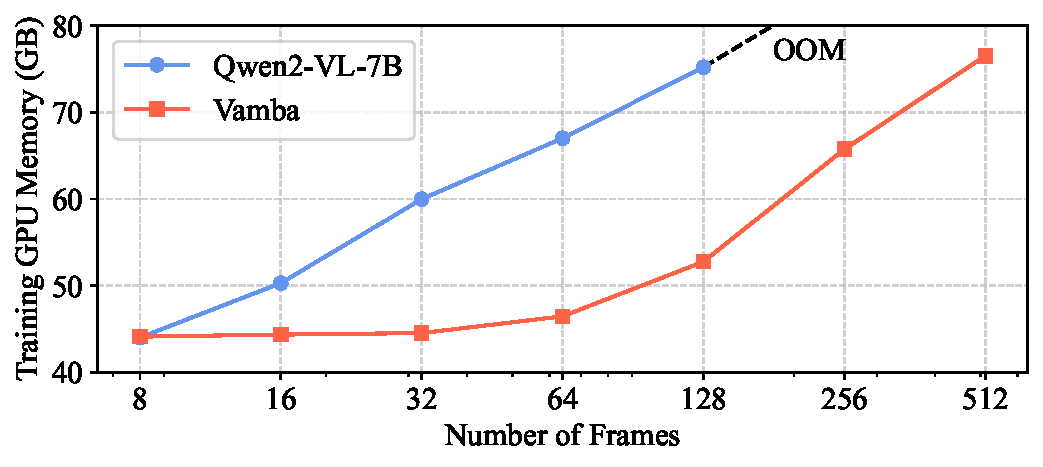
\includegraphics[width=\linewidth]{figures/train_memory.pdf}
        \label{fig:train_memory}
    \end{subfigure}
    
    \vspace{-1.5em}
    
    \begin{subfigure}[b]{1\linewidth}
        \centering
        \caption{Training Runtime Comparison (time for 1 training step)}
        \vspace{-2pt}
        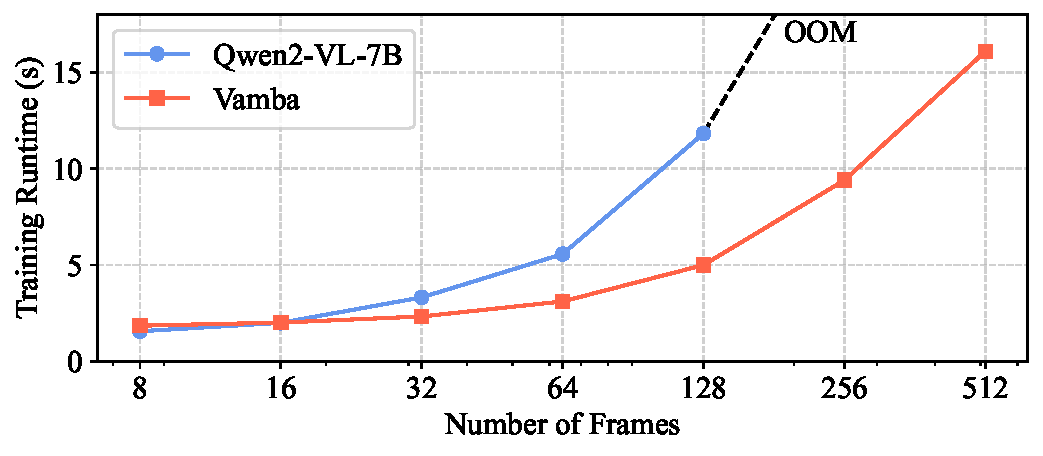
\includegraphics[width=\linewidth]{figures/train_runtime.pdf}
        \label{fig:train_runtime}
    \end{subfigure}
    \vspace{-3.5em}
    \caption{Comparison of training GPU memory usage and runtime per training step between Qwen2-VL-7B and \model.}
    \label{fig:efficiency_main}
    \vspace{-1em}
\end{figure}


\subsection{Runtime Efficiency Analysis}
To understand our model’s runtime efficiency gains over the baseline transformer-based LMM (Qwen2-VL-7B), we conduct an efficiency analysis for both training and inference. For model training, we ensure a consistent training environment by using 8 NVIDIA A800 80G GPUs for both models. All input videos are resized to a resolution of $640\times360$, and a batch size of 1 is maintained on each GPU. We apply standard optimization methods such as Flash-Attention 2 \cite{dao2023flashattention}, DeepSpeed ZeRO-3 \cite{rajbhandari2020zero} and gradient checkpointing \cite{chen2016training} for both models. Based on different numbers of input frames, we measure the average GPU memory across 8 GPUs and the runtime per training step during training. As shown in Figure~\ref{fig:train_memory}, although \model and Qwen2-VL-7B share the same vision encoder design and generate vision tokens of identical sequence lengths, our model requires over 50\% less training memory when processing videos with more than 16 frames. This efficiency gain allows us to handle a larger number of video frames during training (512 vs. 128). Furthermore, as depicted in Figure~\ref{fig:train_runtime}, our efficient design also accelerates model training, achieving nearly twice the speedup per training step when working with more than 64 frames.

For model inference, we focus on the pre-fill stage and analyze GPU memory usage and FLOPs for both models. All measurements are conducted on an input video with a resolution of $640\times 360$. As shown in Figure~\ref{fig:memory}, \model requires slightly more GPU memory than Qwen2-VL-7B when the number of input frames is low (fewer than 32 frames), due to the additional $\sim$3B parameters in its cross-attention and Mamba layers. However, \model's memory usage increases more slowly as the frame increases, allowing it to handle four times as many frames on a single NVIDIA A800 80G GPU compared to Qwen2-VL-7B (256 vs. 1024). Regarding computational cost, \model reduces FLOPs by 30\% to 50\% during inference (Figure~\ref{fig:flops}), demonstrating a significantly lower complexity than its transformer-based LMM counterparts.



\begin{figure}[t!]
    \centering
    
    \begin{subfigure}[b]{1\linewidth}
        \centering
        \caption{Pre-filling GPU Memory Usage Comparison}
        \vspace{-2pt}
        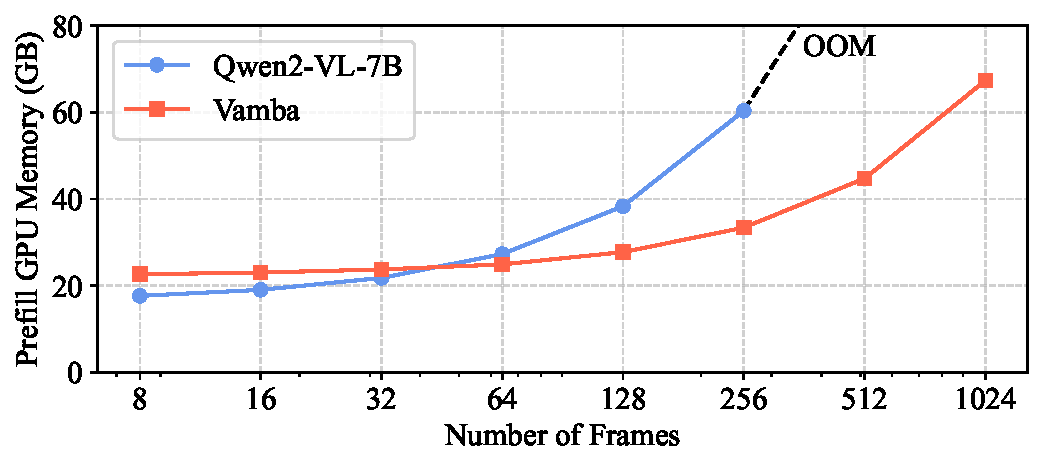
\includegraphics[width=\linewidth]{figures/memory.pdf}
        \label{fig:memory}
    \end{subfigure}
    
    \vspace{-1.5em}
    
    \begin{subfigure}[b]{1\linewidth}
        \centering
        \caption{Pre-filling FLOPs Comparison (measured using \texttt{calflops})}
        \vspace{-2pt}
        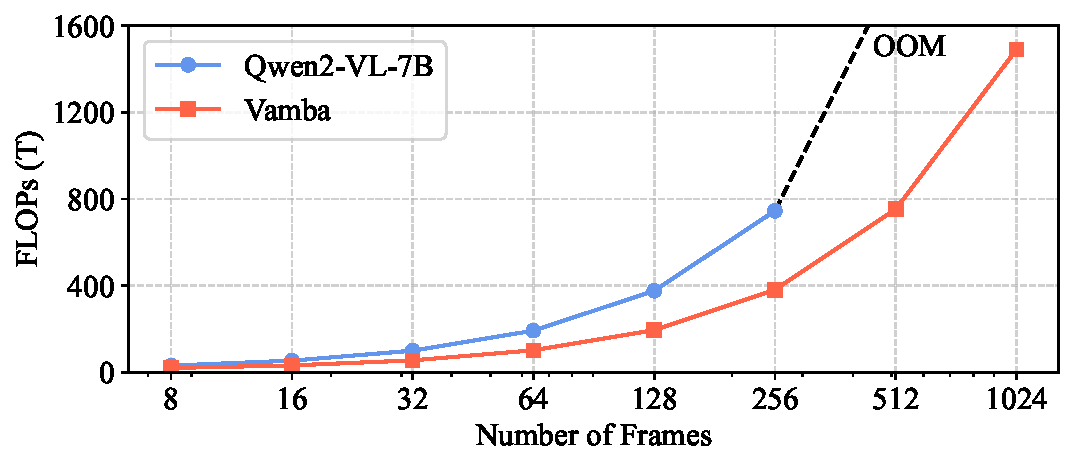
\includegraphics[width=\linewidth]{figures/flops.pdf}
        \label{fig:flops}
    \end{subfigure}
    \vspace{-3.5em}
    \caption{Comparison of GPU memory usage and FLOPs between Qwen2-VL-7B and \model during inference.}
    \label{fig:efficiency_main}
    \vspace{-1em}
\end{figure}


\begin{figure*}[ht!]
  \centering
  
\includegraphics[width=1.0\textwidth]{figures/case_study.pdf}
  \vspace{-2em}
  \caption{Qualitative comparison between \model and efficient LMM baselines. \textcolor{red}{Red text} denotes incorrect responses, while \textcolor{deepgreen}{green text} highlights the correct responses by our \model.}
  \label{fig:case_study}
  \vspace{-1.5em}
\end{figure*}


\subsection{Case Study}
In this section, we perform a case study for Video-XL and \model using different video inputs and show the results in Figure~\ref{fig:case_study}. The ``cookie'' example focuses on object property identification in a long video (36 minutes). Video-XL incorrectly identifies the cookie colors as green and white, possibly due to the video also containing scenes for making other desserts (e.g. white ice cream in the frame highlighted in red). On the other hand, \model more accurately describes them as green and brown. In the ``magic trick'' example, Video-XL misinterprets the rubber band as a green ring, whereas \model correctly describes the performer manipulating the rubber band around their fingers, making it appear to pass through. These comparisons highlight how \model is better at retrieving relevant events in long videos and capturing fine-grained visual details and actions.


